\documentclass[
  captions=tableheading,
  bibliography=totoc, 
  titepage=firstiscover,
]{scrartcl}

\usepackage{blindtext} %neuer input

\usepackage{longtable} % Tabellen über mehrere Seiten

\usepackage[utf8]{inputenc} %neuer input

\usepackage{scrhack}

\usepackage[aux]{rerunfilecheck} %Warnung falls nochmal kompiliert werden muss

\usepackage{fontspec} %Fonteinstellungen

\recalctypearea{}

\usepackage[main=ngerman]{babel} %deutsche Spracheinstellung

\usepackage{ragged2e} %neuer input

\usepackage{amsmath, nccmath}

\usepackage{amssymb} %viele mathe Symbole

\usepackage{mathtools} %Erweiterungen für amsmath


\DeclarePairedDelimiter{\abs}{\lvert}{\rvert}
\DeclarePairedDelimiter{\norm}{\lVert}{\rVert}

\DeclarePairedDelimiter{\bra}{\langle}{\rvert}
\DeclarePairedDelimiter{\ket}{\lvert}{\rangle}

\DeclarePairedDelimiterX{\braket}[2]{\langle}{\rangle}{
#1 \delimsize| #2
}

\NewDocumentCommand \dif {m}
{
\mathinner{\symup{d} #1}
}


\usepackage[
  math-style=ISO,
  bold-style=ISO,
  sans-style=italic,
  nabla=upright,
  partial=upright,
  warnings-off={
    mathtools-colon,
    mathtools-overbracket,
  },
]{unicode-math}

\setmathfont{Latin Modern Math}
\setmathfont{XITS Math}[range={scr, bfscr}]
\setmathfont{XITS Math}[range={cal, bfcal}, StylisticSet=1]


\usepackage[
  locale=DE,
  separate-uncertainty=true,
  per-mode=reciprocal,
  output-decimal-marker={,},
]{siunitx}

\usepackage[autostyle]{csquotes} %richtige Anführungszeichen

\usepackage{xfrac}

\usepackage{float}

\floatplacement{figure}{htbp}

\floatplacement{table}{htbp}

\usepackage[ %floats innerhalb einer section halten
  section,   %floats innerhalb er section halten
  below,     %unterhalb der Section aber auf der selben Seite ist ok
]{placeins}

\usepackage[
  labelfont=bf,
  font=small,
  width=0.9\textwidth,
]{caption}

\usepackage{subcaption} %subfigure, subtable, subref

\usepackage{graphicx}

\usepackage{grffile}

\usepackage{booktabs}

\usepackage{microtype} %Verbesserungen am Schriftbild

\usepackage[
backend=biber,
]{biblatex}

\addbibresource{../lit.bib}

\usepackage[ %Hyperlinks im Dokument
  german,
  unicode,
  pdfusetitle,
  pdfcreator={},
  pdfproducer={},
]{hyperref}

\usepackage{bookmark}

\usepackage[shortcuts]{extdash}

%\usepackage{warpcol}


\begin{document}
    \title{ATP Übungsblatt 9}
    \author{  
    Tobias Rücker\\
    \texorpdfstring{\href{mailto:tobias.ruecker@tu-dortmund.de}{tobias.ruecker@tu-dortmund.de}
    \and}{,} 
    Paul Störbrock\\
    \texorpdfstring{\href{mailto:paul.stoerbrock@tu-dortmund.de}{paul.stoerbrock@tu-dortmund.de}}{}
    }
\maketitle
\center{\Large Abgabegruppe: \textbf{Mittw. 10-12 Uhr}}
\thispagestyle{empty}

\newpage
\tableofcontents
\thispagestyle{empty}
\newpage

\setcounter{page}{1}

\section{Aufgabe 28}

\begin{figure}[H]
    \centering
    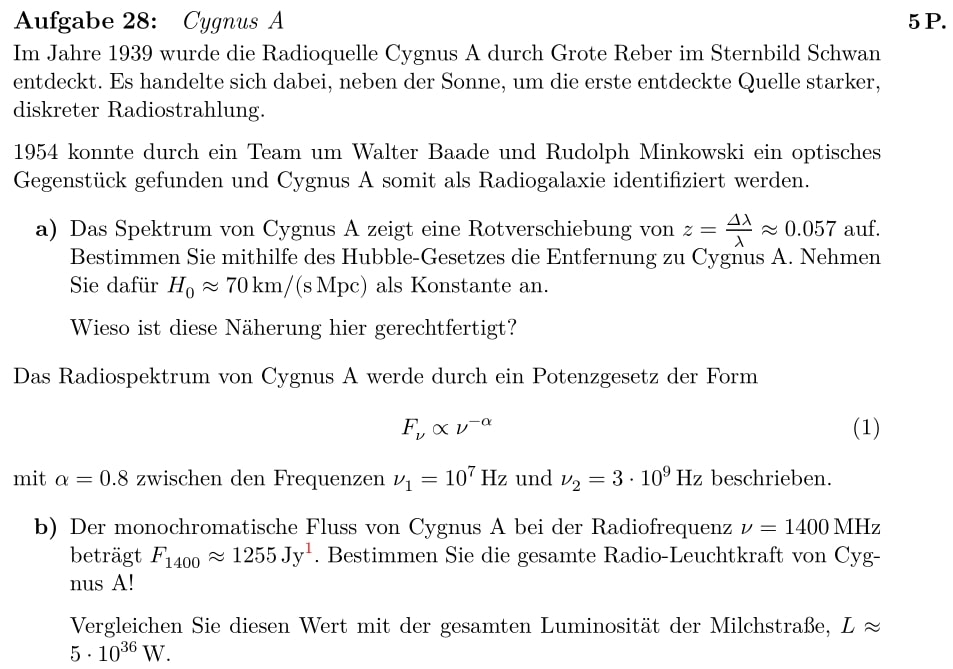
\includegraphics[width=\textwidth]{images/Aufgabe28.jpg}
\end{figure}

\subsection{a)}

\subsection{b)}

\section{Aufgabe 29}

\begin{figure}[H]
    \centering
    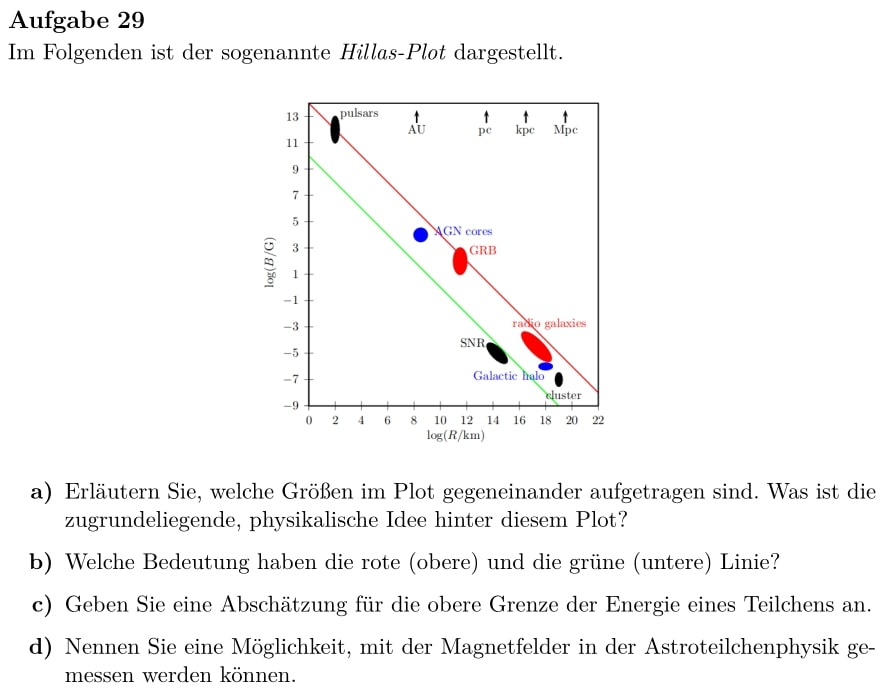
\includegraphics[width=\textwidth]{images/Aufgabe29.jpg}
\end{figure}

\subsection{a)}

\subsection{b)}

\subsection{c)}

\subsection{d)}

\section{Aufgabe 30}

\begin{figure}[H]
    \centering
    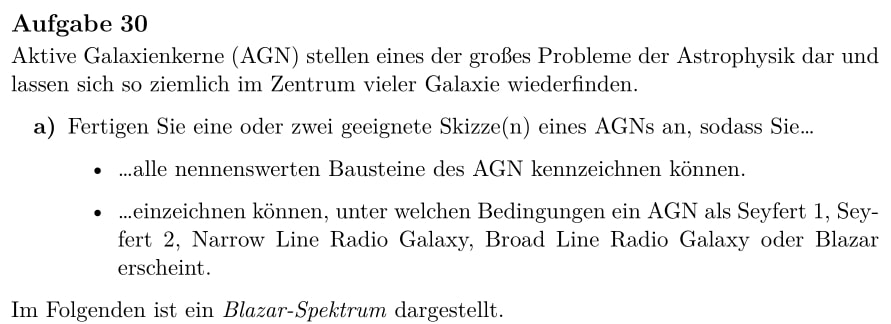
\includegraphics[width=\textwidth]{images/Aufgabe30a.jpg}
\end{figure}

\begin{figure}[H]
    \centering
    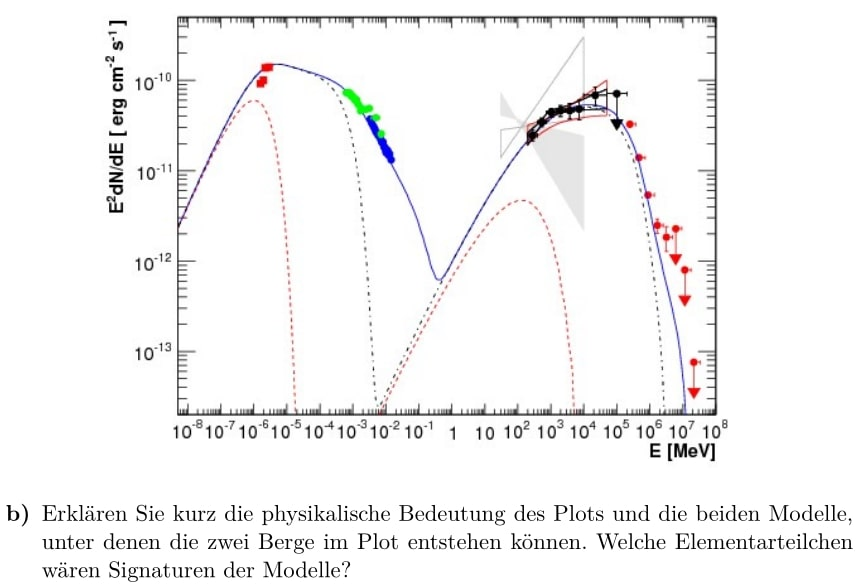
\includegraphics[width=\textwidth]{images/Aufgabe30b.jpg}
\end{figure}

\subsection{a)}

\begin{figure}[H]
    \centering
    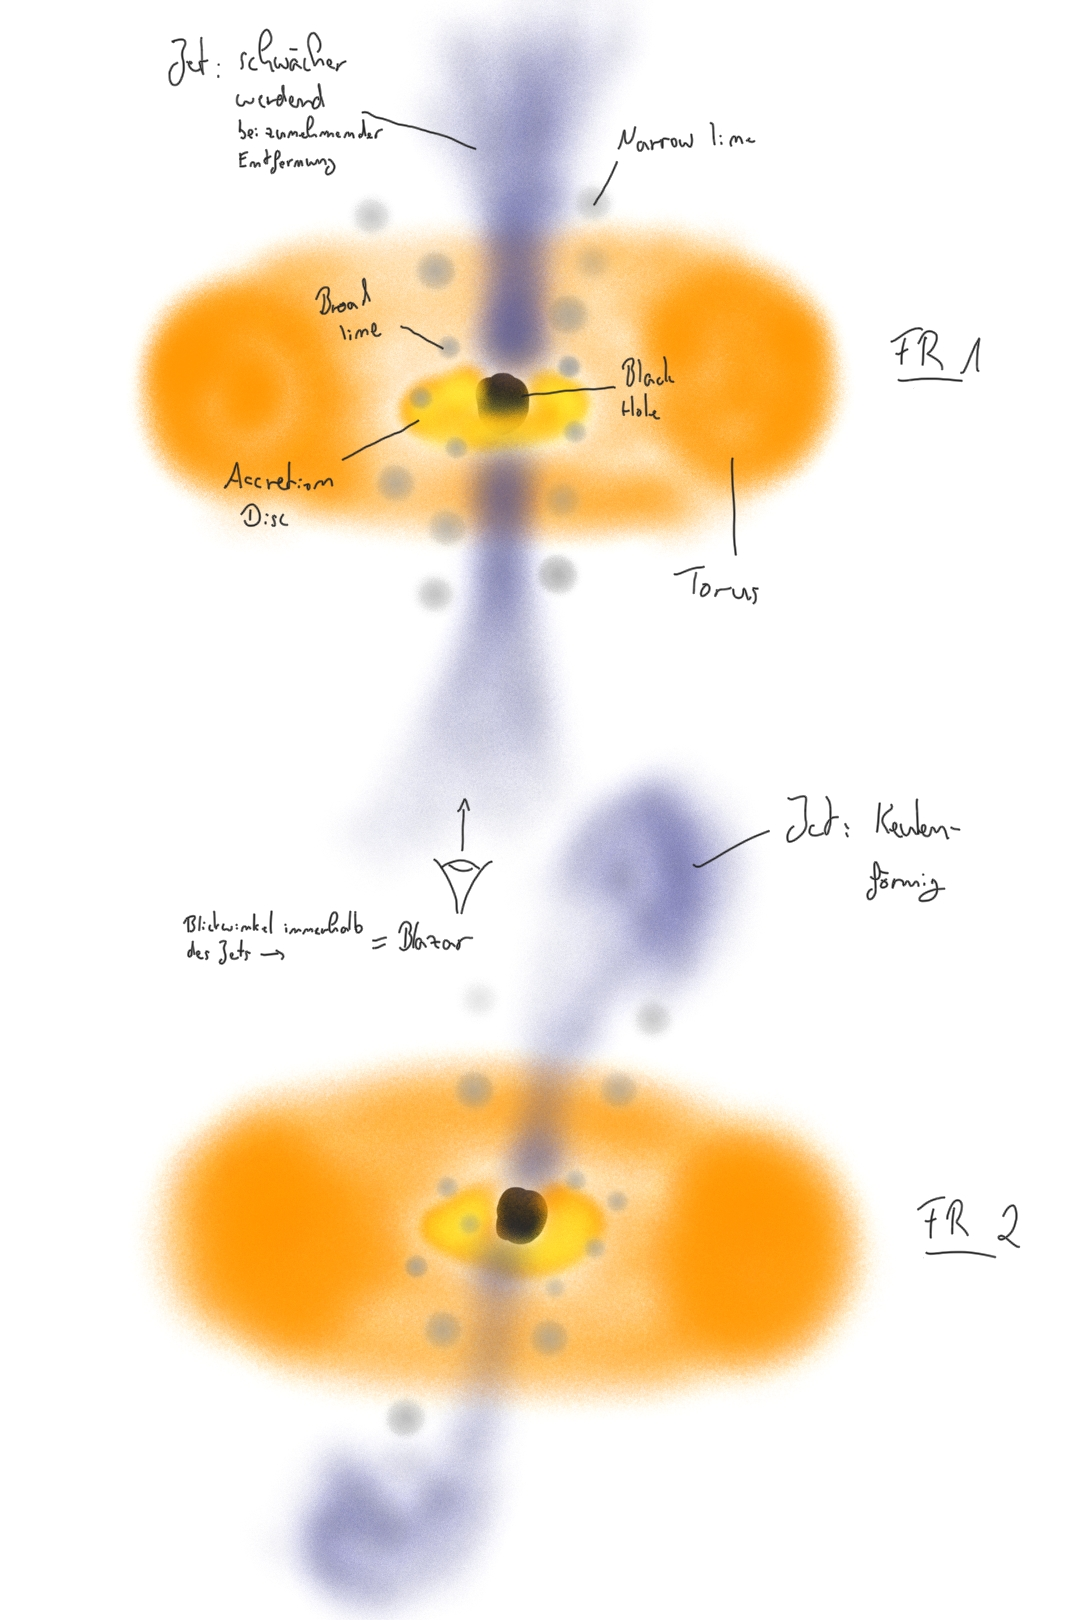
\includegraphics[width=\textwidth]{images/30a.jpg}
\end{figure}

\subsection{b)}
Der Plot stellt das Energiespektrum der Photonen eines AGN's dar, dessen Jet in Richtung der Erde zeigt.
Der jet zeigt dabei zwei charakteristische Höcker, welche auf zwei dominierende Emissionsvorgänge
schließen lässt. Diese ist von nicht-thermischer Strahlung dominiert, kommt von Galaxien mit starken
Radiosignalen und der genaue physikalische Mechanismus dahinter ist experimentell noch unbestätigt.\\
Ein Modell, welches versucht diesen Plot zu beschreiben ist das SSC/EC -Modell: \\
Da wird der 1. Bump durch die Synchrotron-Emission der Elektronen entsteht,
während der Hochenergie-Bump durch inversen Compton Prozess entsteht.
Dabei unterscheiden sich SSC und EC in der Hinsicht, woher die Photonen für
den inversen Compton-prozess kommen. Bei EC Modell wird von externen Photonen von zum 
Beispiel dem Staubtorus oder der Akkretionsscheibe ausgegangen, während beim SSC
Modell die Photonen aus der Synchrotron-Emission mit den Elektronen wechselwirken.\\

Ein anderes Modell bildet das Proton-Blazar-Modell:\\
Hier kommt der erste Bump aus dem gleichen Prozess wie zuvor. Der Hochenergie-Bump 
setzt sich hier aus verschiedenen Beiträgen zusammen. Einer kommt
dabei aus Gammaphotonen aus $\pi ^0$-Zerfällen , welche aus WW von 
Protonen und Photonen kommt.
Ein weiterer Beitrag liefern die Synchrotron-Emission von Protonen und Myonen, wobei
die Myonen aus $\pi ^{+/-}$-Zerfällen stammen.\\

Aus dem $\pi ^+$ -Zerfall entstehen Neutrinos, welche als Botenteilchen für das
Proton-Blazar-Modell gemessen werden könnten.

\end{document}